%!TEX root = ../thesis.tex
%Adding the above line, with the name of your base .tex file (in this case "thesis.tex") will allow you to compile the whole thesis even when working inside one of the chapter tex files

\chapter{Appendix}

\label{app:1}

If we assume the herringbones are due to the shock drift acceleration process then the velocity upon a reflection from the shock is
\begin{equation}
v_{r,||} = 2v_{shock}\mathrm{sec}\,\theta_{Bn} - v_{i,||}
\end{equation}
where $v_{r,||}$ is the reflected parallel velocity of the particle, $v_{i,||}$ is the incident parallel velocity of the paticle, $v_{shock}$ is the shock velocity, and $\theta$ is the angle between upstream $B-$field and shock normal $n$. Taking the shock speed to be the speed of the 150\,MHz radio source, $550\times10^3$\,m\,s$^{-1}$, and $v_{i,||}$ to be the thermal speed of an electron 
\begin{equation} 
v_{thermal} = \sqrt{ \frac{3k_bT}{m_e} }
\end{equation}
At $1\times10^{6}$\,K, $v_{thermal} = v_{i,||} = 6.7\times10^6$\,m\,s$^{-1}$. Now, the herringbone electron speed 0.15\,c, this is the reflected speed $v_{r,||}$ in equation A1. Rearranging A1 we get
\begin{equation}
\theta_{Bn} = \mathrm{sec}^{-1}\bigg( \frac{1}{2}\frac{v_{r,||} +  v_{i,||} }{v_{shock}}\bigg)
\end{equation}
Substituting the above values we get $\theta_{Bn}=88^{\circ}$. Independent verification of a quasi-perpendicular shock orientation!



\section{Radio burst intensity}


\begin{equation}
\Phi_F \approx 72\sqrt{3}   \frac{\gamma_{L^{'}}}{\gamma_S}   \frac{v_e^3}{c^3}   \frac{v_b}{\Delta v_b}   \frac{e^{-u_c^2}}{u_c\sqrt{\pi}}  \zeta_F
\end{equation}
\begin{equation}
\Phi_H \approx \frac{18\sqrt{3}}{5\gamma_t}   \sqrt{\frac{m_i}{\gamma_t m_e}}  \frac{v_e^3 v_b^3}{c^5} \frac{v_b}{\Delta v_b}\zeta_H
\end{equation}
the expression involving $u_c$ represent an \textquoteleft escape factor' for the fundamental taking into account absorption and scattering of the radiation. $ \frac{\gamma_{L^{'}}}{\gamma_S} $ is the ratio of the damping rates of the product waves out of processes in equations~\ref{eqn:harm} and \ref{eqn:fund}. The $\zeta$ terms are the fractions of Langmuir waves that are kinematically able to contribute to the fundamental or harmonic emission, given by

\begin{equation}
\zeta_F  \approx \mathrm{exp} \bigg[  -\frac{4\gamma_t m_e}{45 m_i}    \bigg(\frac{v_b}{\Delta v_b}\bigg)^2   \bigg(  \frac{3}{2}  \sqrt{\frac{m_i}{\gamma_t m_e}} - \frac{v_b}{v_e}  \bigg)^2    \bigg]
\end{equation}

\begin{equation}
\zeta_H \approx \frac{c}{2v_b} \sqrt{\frac{\pi}{6}} \frac{\beta \Delta v_b}{v_b}
\Bigg[  \mathrm{erf}\Bigg(     \frac{ \frac{v_e\sqrt{3}}{c}  + \frac{2}{3} \sqrt{\frac{\gamma_t m_e}{m_i}}  }  {\frac{v_e}{v_b} \frac{\beta \Delta v_b}{v_b} \sqrt{2} }   \Bigg)     +   \mathrm{erf}\Bigg(     \frac{ \frac{v_e\sqrt{3}}{c}  - \frac{2}{3} \sqrt{\frac{\gamma_t m_e}{m_i}}  }  {\frac{v_e}{v_b} \frac{\beta \Delta v_b}{v_b} \sqrt{2} }   \Bigg)   \Bigg]
\end{equation}
where erf is the error function. 


\section{Band-splitting}
Using a ploytropic index of $\gamma=5/3$ (monatomic) means the shock compression can be no more than a factor of 4. Another extremely important fact arising from this is that magnetic compression can also be no greater than 4 i.e., from equation 4(b) $B_{2}/B_{1}=\chi$. $\chi<4$ has consequences for the shock drift acceleration mechanism and provides an upper limit to the particle energy gain

may also provide an upper limit to the level of band splitting in type II radio bursts (since this effect is thought to be related to the emission induced up/downstream of the shock). Although the maximum compression ration of 4 was derived from the roots of the quadratic for $\chi$ for the perpendicular shock, a similar analysis for the much more general oblique shock also leads to the same result. The density compression and tangential magnetic compression can be no more than a factor of $(\gamma+1)/(\gamma-1)$ for any MHD shock. 

%In either the perpendicular case or the general 2D oblique case a polynomial expression for the compression ratio (such as (6)) may be derived. The general oblique shock case requires extra terms in the polynomial such as $M_{A},\beta,\gamma,\theta_{Bn},\theta_{vn}$ ($\theta_{Bn}$ is the angle between shock normal and magnetic field, and $\theta_vn$ is the angle between shock normal and plasma flow). 
Polynomials such as (6) are extremely useful, and can lead to simple expressions for the Alfv\'{e}nic-Mach number in terms of $\chi$, in this case
\begin{equation}
M_{A}=\sqrt{\frac{\chi(\chi+5+5\beta)}{2(4-\chi)}} 
\end{equation}
for a perpendicular shock. If the shock speed and compression ratio are known, this equation provides a means of measuring the Alfv\'{e}n speed in the shock medium. 

This technique is exploited in the analysis of type II radio bursts. As the shock propagates into the corona it emits EM radiation at the local plasma frequency (1) (see section 4), and since the density drops as the shock travels into the heliosphere, so too does the frequency of emission. From frequency drift rate an estimate of shock speed is possible. If band splitting of the emission is present this is interpreted as emission from upstream and downstream of the shock, which provides a diagnostic of upstream/downstream densities via (1) and hence an estimate of $\chi$ \citep{vrsnak2002}. However, use of (8) in calculating Mach number and Alfv\'{e}n speed in the corona has some clear shortcomings such that it clearly ignores any dependency of the angle between magnetic field, velocity vector and shock normal i.e., (8) only applies to a purely perpendicular shock.

The general oblique shock case requires extra terms in the polynomial such as $\theta_{Bn}$ and $\theta_{vn}$ ($\theta_{Bn}$ is the angle between shock normal and magnetic field, and $\theta_{vn}$ is the angle between shock normal and plasma flow). For the oblique case the polynomial becomes
\begin{equation}
(A^2-\chi)^2\bigg[A^2 - \frac{2\chi S^2}{\chi+1-\gamma(\chi-1)}\bigg]\\
-\chi k^2A^2\bigg[\frac{2\chi - \gamma(\chi-1)}{\chi+1- \gamma(\chi-1)}A^2 -\chi\bigg]=0
\end{equation}
where $A=\frac{M_A\mathrm{cos}\theta_{vn}}{cos(\theta_{Bv}-\theta_{bn})}$,  $S=\frac{c_s}{v_A}$, $k=\mathrm{tan}(\theta_{vn}-\theta_{Bv})$ \footnote{$\theta_{Bv}$ is angle between magnetic field and velocity vector, it has a simple relationship with $\theta_{Bn}$} 
\citep{kabin2001}. Equation (6) is a quadratic of variable $\chi$, the more general equation (9) is a cubic equation for $\chi$, the roots of which give the compression for the oblique case. Since it is a function of $M_A$, $\theta_{vn}$, and $\theta_{bv}$, $\chi$ may have a range of values depending not only on Mach number but also shock orientation. Figure 2 illustrates the broad range in compressions of 0$<\chi<$3.5 across the shock depending on both flow and magnetic field orientation with respect to the shock normal, and in this case $M_A=2.5$. 
%\begin{figure}[h!]
%\includegraphics[scale=0.5, angle=270,trim =  3cm 0cm 4cm 0cm]{data/vary_thetaVn_thetaBn_mach2_5.pdf}
%\caption{Image and surface plot of compression ratio (from the solutions of (9)) as a function of $\theta_{vn}$ and $\theta_{Bn}$, with an Alfv\'{e}n Mach number of 2.5. The range of compressions is from 0 to 3.5 depending on the orientation of the magnetic field and velocity vectors with respect to the shock normal. Any discontinuities or sharp jumps are an indication of where the solutions to (9) are multi-valued.}
%\label{fig:vary_thetaVn_thetaBn_mach2_5}
%\end{figure}
This is a very general case, however, permitting any angle of orentation of $B$ and $v$. Since type II bursts are thought to be from shocks that are quasi perpendicular, this places restriction on the values for $\theta_{vn}$, and $\theta_{Bn}$, especially when the flow is considered to be head-on i.e. $\theta_{vn}=0^{\circ}$. Therefore in the quasi-perpendicular case their is a tighter constraint on the amount of compression across the shock. Further constraining the Mach number to a limited range of values puts quite a limiting range on the compression ratio, and hence a limiting range of band splitting of type II radio bursts since $f_{plasma}\approx9000\sqrt{n_e}$, hence
\begin{equation}
\delta_{bs} \equiv \frac{f_{upper}}{f_{lower}} \approx \sqrt{ \frac{ n_{e,d} }{ n_{e,u} } }=\sqrt{\chi}
\end{equation}
where $n_{e,d}$ and $n_{e,u}$ are downstream and upstream plasma number densities, and $\delta_{bs}$ is the ratio of upper to lower band frequencies, $f_{upper}$ and $f_{lower}$ respectively, in a split radio burst. Figure 3 shows the expected range in band splitting ($\delta_{bs}=\sqrt{\chi}$) for a type II given a range in Alfv\'{e}n Mach numbers $1<M_A< 4$, and quasi-perpendicular magnetic field orientations $45^{\circ}<\theta_{Bn}<90^{\circ}$. 
\begin{figure}[h!]
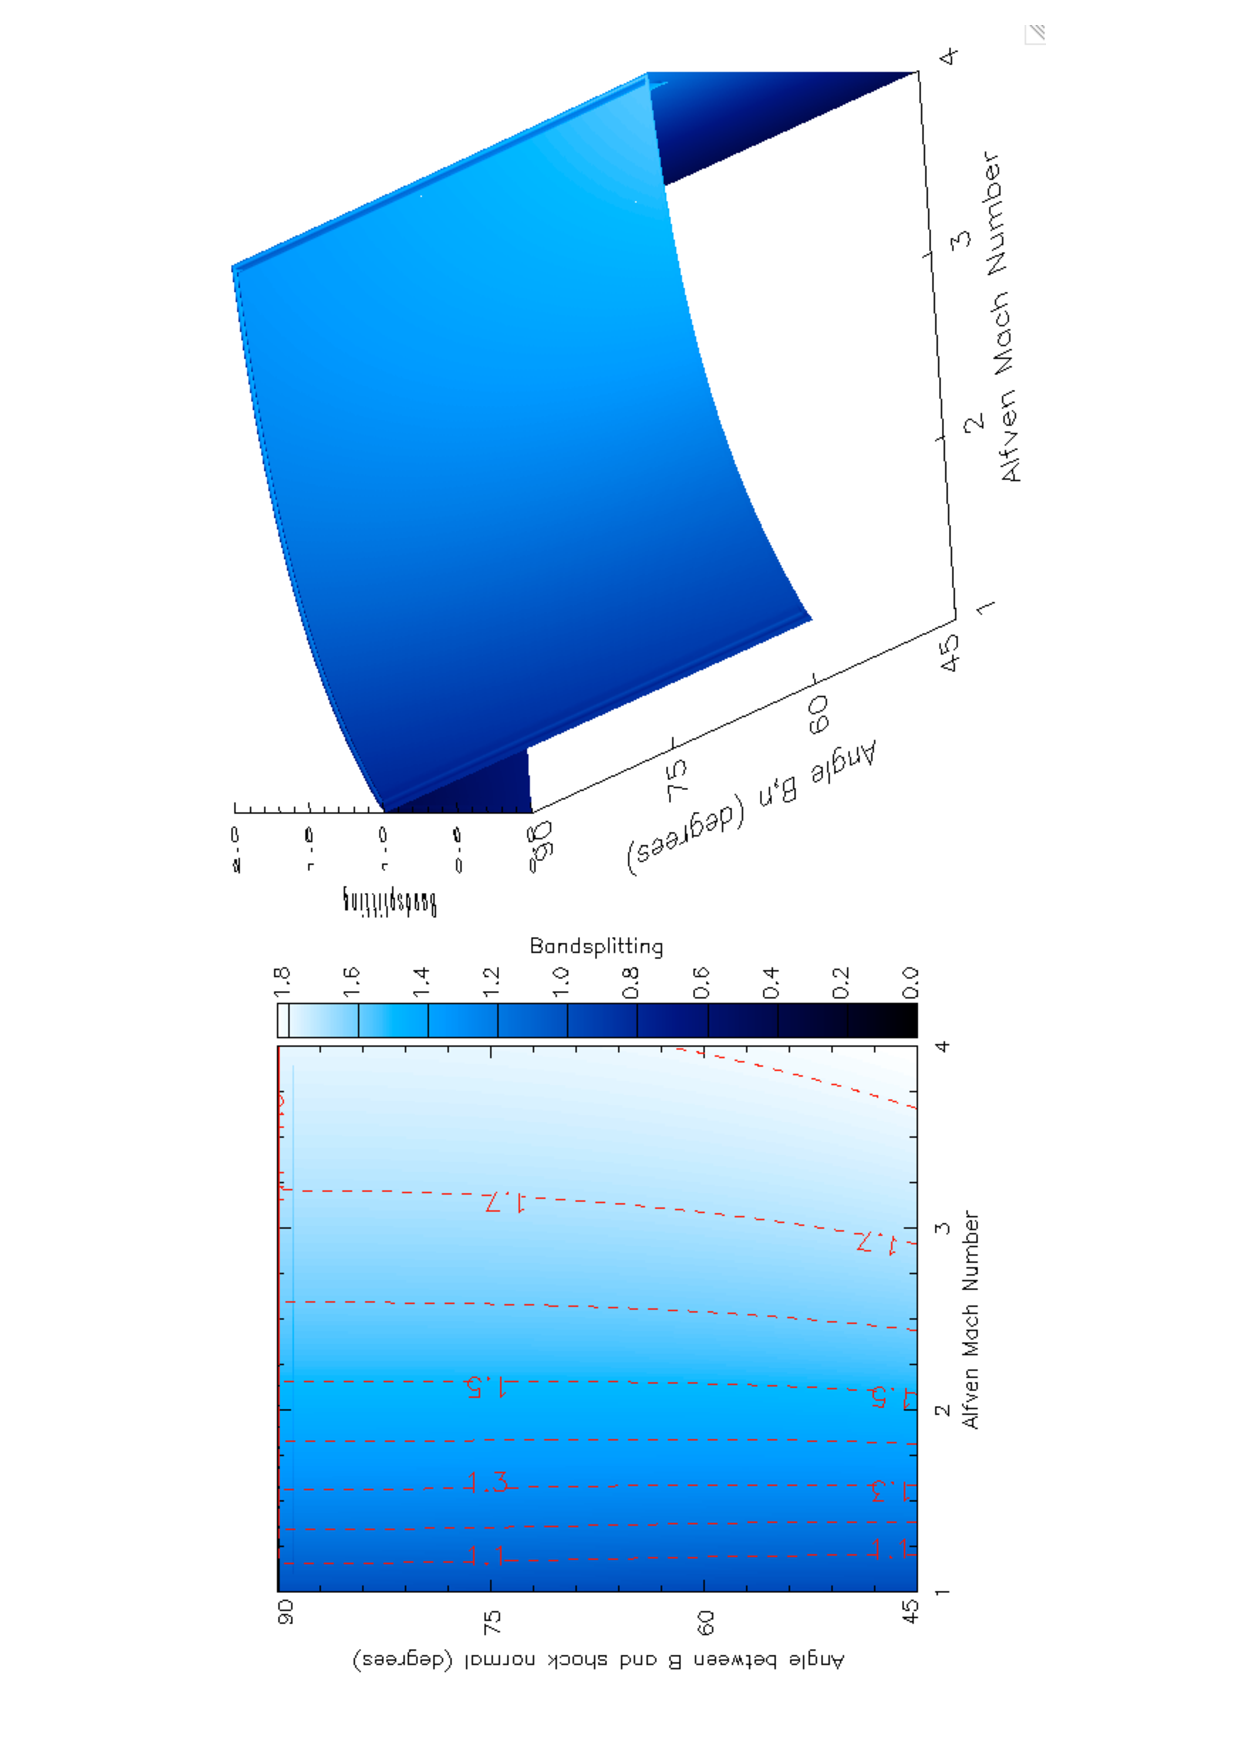
\includegraphics[scale=0.5, angle=270,trim =  3cm 0cm 4cm 0cm]{images/MHD_vary_mach&thetaBn.pdf}
\caption[Band-splitting as a function of Mach number]{Predicted band splitting ratio $\delta_{bs}$ as a function of Mach number and magnetic field orientation with respect to shock normal. Flow is anti-parallel to shock normal (head-on). Both image and surface are shown, left and right respectively. On the left, the red contours show specific values of of band-splitting. Note that for small mach numbers the level of band splitting is independent of magnetic field orientation. It is only at Mach numbers greater than $\sim$2.1 that the B-field orientation becomes important.}
\label{fig:MHD_vary_mach&thetaBn}
\end{figure}
This analysis shows that for a quasi-perpendicular shock the theoretically predicted range in type II band-spliting is $1<\delta_{bs}<1.8$. Such an upper limit to the level of band-splitting seems excessive and is probably due to a large upper limit to the Mach number being used to calculate the compression ratio. This is especially relevant in the low corona where Alfv\'{e}n speed can be quite large, making it difficult for a CME or blast wave to drive a shock at $M_A=4$. Also, given a typical band-splitting ratio of $\delta_{bs}=1.21\pm0.7$ at metric wavelengths \citep{vrsnak2004}, this would indicate typical Alfv\'{e}n-Mach number of $\sim\,1.5$ in the low corona. This seems reasonable, however Mach numbers of $\sim$3 are possible, and figure 3 would suggest a possible band-split ratio of $\delta_{bs}\sim1.7$ for such a Mach number. Such a level of band-splitting seems very unlikely, suggesting a quasi-perpendicular shock with a head on flow is a limiting case. More likely is a quasi-perpendicular shock with a flow orientation $\theta_{vn}\neq0$. For example if $\theta_{Bn}=90^{\circ}$ and $\theta_{vn}=45^{\circ}$ then band splitting can be $\delta_{bs}\sim\,1.5$ for $M_A$=3, which is under the upper limit of observed type II band-split ratios of $\sim\,1.58$. Allowing $\theta_{vn}\neq0$ can allow larger, more realistic Mach numbers to produce smaller and more realistic bandsplitting.


It is clear that the distribution in the level of band splitting in type II radio bursts depends not only on Mach number but the relative orientations of flow and magnetic field with respect to shock normal. A statistical analysis could possibly give an observationally predicted distribution in $\theta_{Bn}$ (provided $M_A$ is known) that would confirm the quasi-perpendicularlity of type II-generating shocks.

\section{EUV and pB Density Measurements}\label{app:densities}

Electron densities were calculated from emission measure maps derived using the SDO/AIA�s six coronal filters and the method of \citep{asch2013}. The method starts by reconstructing the differential emission measure $dEM/dT (DEM)$, using the intensity of the six SDO/AIA filters for each pixel. The DEM is a measure of the amount of plasma along the line-of-sight (LOS) that contributes to the emitted radiation in the temperature range $T$ to $T +dT$ \citep{craig1976}. Once the EM was obtained, the plasma electron density can be calculated estimating an effective length of the LOS of the emitting plasma. The 2D $EM(r, \phi)$ map, which is a function of heliocentric distance $r$ and latitude, can then be written as
\begin{eqnarray}
EM(r, \phi) &=& \int \bigg( \frac{dEM(r,\phi)}{dT} \bigg) dT \\
			  &=& \int <N_e^2> ds
\end{eqnarray}

Knowing the line-of-sight length, $s$, the density of the emitting plasma can be obtained from the EM,
\begin{equation}
N_e(r, \phi) =\sqrt{  \frac{EM(r, \phi)}{s(r)}  }
\end{equation}
The LOS length was calculated using a geometrical method used widely in stellar atmospheres \citep{menzel1936}. The LOS length s changes at different distance $r$ and contributes to the intensity of the emitting plasma measured by the observer. This gives the LOS using an asymptotic series expansion in the form
\begin{equation}
S\approx \sqrt{H\pi r}
\end{equation}
where $H$ is the scale height. Using a typical coronal temperature of 2\,MK the scale height $H$ is of the order of $9\times10^9$\,cm and the LOS is in the order of $4\times10^{10}$\,cm. The LOS length does not change significantly in the 1--1.3\,$R_{\odot}$ range. 

As for the polarized brightness measurements, the density diagnostic is through the use of coronagraph images and the Thomson scattering theory outlines in Chaoter. The method involves using the coronagraph data to extract polarized brightness measurements as a function of height i.e., along a radial trace in the coronagraph images. A polynomial is then fit to this data
\begin{equation}
I_t - I_r =\sum_s k_s x^{-s}
\end{equation} 
where $I_t - I_r$ is the polarized brightness, and $x$ is the radial position in the corona, $r$, projected onto the plane of sky. \citet{vdeh50} showed that by use of the van de Hulst coefficients the electron density along the same radial trace can be expressed as 
\begin{equation}
N(r) = \frac{1}{C\{A(r) - B(r)\}}\sum_s \frac{k_s}{a_{s+1}} r^{-s} \, \,\,\,\,\, \textrm{where} \,\,\,\,\, a_n=\frac{\pi}{2^{n+1}}\frac{n!}{(1/2n!)^2}
\end{equation}
here $C$ is constant equal to $\frac{3}{4}\times1R_{\odot}\times \sigma_T$; $\sigma_T$ is the Thomson scattering cross section and $A(r)$ and $B(r)$ are the van de Hulst coefficients (see Chapter 4). Here, the same $k_s$ produced from the polarized brightness fit are used to calculate $N(r)$. 

